\documentclass{standalone}
\usepackage{tikz}
\usetikzlibrary{patterns}
\usetikzlibrary{positioning}
\usetikzlibrary{patterns, positioning}
\usetikzlibrary{shapes.misc}
\usepackage[outline]{contour}
\contourlength{1.5pt} 


\begin{document}
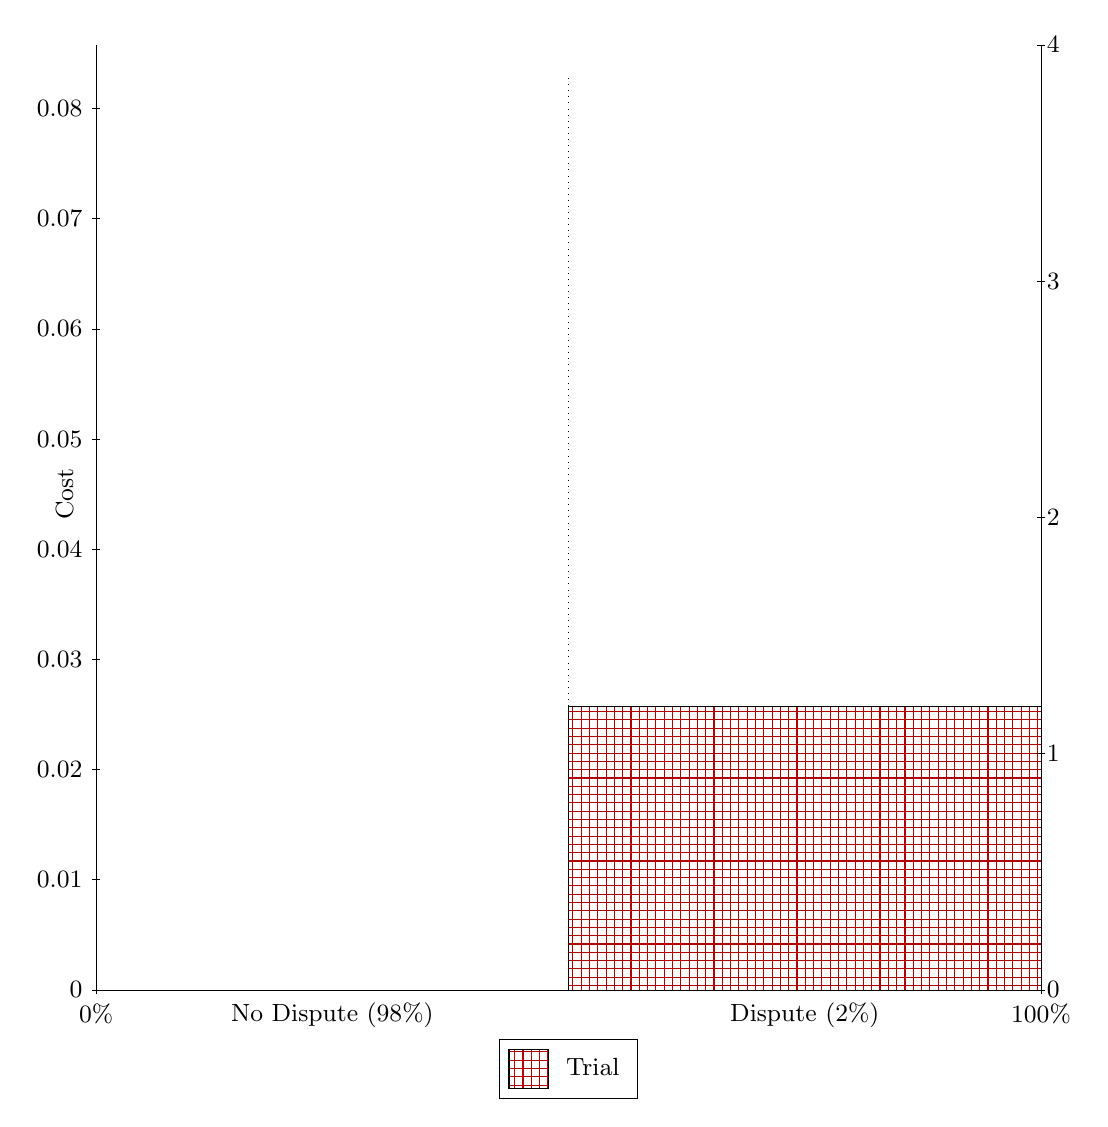
\begin{tikzpicture}
\draw[pattern=grid,            pattern color=red!70!black,draw=black,very thin] (7.5,2.5) rectangle (13.5,6.1);
\draw[black,very thin] (1.5,2.5) -- (1.5,14.5);
\node[font=\small,rotate=90,text=black, anchor=center] at (1.1, 8.7949) {Cost};
\draw[black,very thin] (1.45,2.5) -- (1.55,2.5);
\node[font=\small,text=black, anchor=east] at (1.45, 2.5) {0};
\draw[black,very thin] (1.45,3.8989) -- (1.55,3.8989);
\node[font=\small,text=black, anchor=east] at (1.45, 3.8989) {0.01};
\draw[black,very thin] (1.45,5.2977) -- (1.55,5.2977);
\node[font=\small,text=black, anchor=east] at (1.45, 5.2977) {0.02};
\draw[black,very thin] (1.45,6.6966) -- (1.55,6.6966);
\node[font=\small,text=black, anchor=east] at (1.45, 6.6966) {0.03};
\draw[black,very thin] (1.45,8.0955) -- (1.55,8.0955);
\node[font=\small,text=black, anchor=east] at (1.45, 8.0955) {0.04};
\draw[black,very thin] (1.45,9.4944) -- (1.55,9.4944);
\node[font=\small,text=black, anchor=east] at (1.45, 9.4944) {0.05};
\draw[black,very thin] (1.45,10.893) -- (1.55,10.893);
\node[font=\small,text=black, anchor=east] at (1.45, 10.893) {0.06};
\draw[black,very thin] (1.45,12.292) -- (1.55,12.292);
\node[font=\small,text=black, anchor=east] at (1.45, 12.292) {0.07};
\draw[black,very thin] (1.45,13.691) -- (1.55,13.691);
\node[font=\small,text=black, anchor=east] at (1.45, 13.691) {0.08};

\draw[black,dotted,very thin] (7.5,2.86) -- (7.5,14.14);
\draw[black,very thin] (13.5,2.5) -- (13.5,14.5);
\draw[black,very thin] (13.45,2.5) -- (13.55,2.5);
\node[font=\small,text=black, anchor=west] at (13.45, 2.5) {0};
\draw[black,very thin] (13.45,5.5) -- (13.55,5.5);
\node[font=\small,text=black, anchor=west] at (13.45, 5.5) {1};
\draw[black,very thin] (13.45,8.5) -- (13.55,8.5);
\node[font=\small,text=black, anchor=west] at (13.45, 8.5) {2};
\draw[black,very thin] (13.45,11.5) -- (13.55,11.5);
\node[font=\small,text=black, anchor=west] at (13.45, 11.5) {3};
\draw[black,very thin] (13.45,14.5) -- (13.55,14.5);
\node[font=\small,text=black, anchor=west] at (13.45, 14.5) {4};

\draw[black,very thin] (1.5,2.5) -- (13.5,2.5);
\draw[black,very thin] (1.5,2.45) -- (1.5,2.55);
\node[font=\small,text=black, anchor=north] at (1.5, 2.45) {0\%};
\draw[black,very thin] (13.5,2.45) -- (13.5,2.55);
\node[font=\small,text=black, anchor=north] at (13.5, 2.45) {100\%};

\node[font=\small,text=black,anchor=south] at (4.5, 1.9) {No\ Dispute\ (98\%)};
\node[font=\small,text=black,anchor=south] at (10.5, 1.9) {Dispute\ (2\%)};
\draw (7.5,2.5) node (B) {};
\begin{scope}[align=center]
\matrix[scale=0.5,draw=black,below=0.5cm of B,nodes={draw},column sep=0.1cm]{
\node[rectangle,draw,minimum width=0.5cm,minimum height=0.5cm,pattern=grid,            pattern color=red!70!black]{}; & \node[draw=none,font=\small,text=black]{Trial}; \\\\
};\end{scope}

\end{tikzpicture}
\end{document}